% !TEX options=--shell-escape
\documentclass[12pt]{article}
\usepackage[utf8]{inputenc}
\usepackage{lipsum}
\usepackage{afterpage}
\usepackage{mathtools}
\usepackage{xcolor}
\usepackage[12pt]{extsizes}
\usepackage[english,russian]{babel}
\usepackage{cite}
\usepackage{minted}
\usepackage{amsmath, esint, setspace, fancyhdr, amsfonts, bookmark, blindtext}
\usepackage{graphicx}
\usepackage{subfigure}
\usepackage{titlesec}

\graphicspath{{Figures/}}
\DeclareGraphicsExtensions{.pdf,.png,.jpg}
\usemintedstyle{tango}
\definecolor{dhscodebg}{rgb}{0.95,0.95,0.95}


\setlength{\textheight}{8in}
\setlength{\textwidth}{6.6in}
\setlength{\headheight}{0in}
\setlength{\headsep}{0.2in}
\setlength{\topmargin}{0in}
\setlength{\oddsidemargin}{0in}
\setlength{\evensidemargin}{0in}
\setlength{\parindent}{.3in}

\doublespacing
\renewcommand{\baselinestretch}{1.4} 

\begin{document}
\begin{titlepage}

\begin{center}
Санкт-Петербургский политехнический университет Петра Великого\\
Институт прикладной математики и механики\\
Кафедра прикладной математики\\
\end{center}


\vspace{2.5cm}

\begin{center}
{\large {\bfseries СВОДНЫЙ ОТЧЕТ}}\\

\bigskip \bfseries{Тема:} {\bfseries \emph{Многомерные распределения.\\ Оценки характеристик распределений}}
\end{center}

\vspace{1.5cm}

\begin{flushleft}
Направление: 01.03.02 Прикладная математика и информатика

\vspace{1.5cm}

Выполнил студент гр. 33631/4 \hfill{Камалетдинова Ю.} \\ 

\vspace{0.5cm} Преподаватель \hfill{Баженов А.}
\vspace{1cm}

\end{flushleft}

\vspace{2.7cm}

\begin{center}
Санкт-Петербург\\
2019
\end{center}

\end{titlepage}



\tableofcontents
\addtocontents{toc}{~\hfill\par}
\vfill ~
\setcounter{section}{0}


%%%%%%%%%%%%%%%%%%%%%%%%%%%%%%%%%%%%%%%%%%

\newpage 
\section*{Постановка задачи}
\addcontentsline{toc}{section}{Постановка задачи}
\indent{\indentВ данной лабораторной работе исследуется такой способ представления набора статистических данных как гистограмма. Требуется сгенерировать выборки разного размера для заданных распределений, построить гистограммы и сделать выводы о взаимосвязи функции плотности распределения и функции гистограммы.}


\begin{equation}
	\label{dist:1}
	N(x, 0, 1) = \frac{1}{\sqrt{2\pi}}e^{-\frac{x^2}{2}} \;\text{-- стандартное нормальное}
\end{equation}
 
\begin{equation}
	C(x, 0, 1) = \frac{1}{\pi(1 + x^2)} \;\text{-- Коши} \label{dist:2}
\end{equation}

\begin{equation}
	L(x, 0, \frac{1}{\sqrt{2}}) = \frac{1}{\sqrt{2}}e^{{-\sqrt{2}|x|}} \;\text{-- Лаплас} \label{dist:3}
\end{equation}

\begin{equation} 
	U(x, -\sqrt{3}, \sqrt{3}) = 
    \begin{cases}
        \frac{1}{2\sqrt{3}}, \: |x| \leq \sqrt{3}\\
        \;\; 0, \:\:\:|x| > \sqrt{3}
    \end{cases}
    \;\text{-- равномерное} \label{dist:4}
\end{equation}

\begin{equation}
    P(\lambda) = \frac{e^{-\lambda}}{k!}\lambda^k \;\text{-- Пуассон} \label{dist:5}
\end{equation}

%%%%%%%%%%%%%%%%%%%%%%%%%%%%%%%%%%%%%%%%%%

\section*{Описание метода}
\addcontentsline{toc}{section}{Описание метода}
\indent{\indentДля построения гистограммы разобьем множество возможных значений $\xi$ выбоки на непересекающиеся интервалы $\Delta_j = [t_j, t_{j+1}), \; j=\overline{0, m}; \; t_0=-\infty,\; t_{m+1}=+\infty$. Количество элементов $X$ выборки из объема $n$, попавших в интервал $\Delta_j$, обозначим через $v_j$, то есть $v_j = \sum_{i=1}^{n}{I(X_i \in \Delta_j)}$. По теореме Бернулли при $n\to\infty$}

\begin{equation}
    \label{eq:1}
    v_j/n \to P(\xi \in \Delta_j) = \int_{\Delta_j}f(u)du = |\Delta_j|f(c), \; c \in \Delta_j
\end{equation}

\indent{\indentКусочно-постоянная функция, приведенная ниже, есть нормализованная гистограмма}

\begin{equation}
    \label{eq:2}
	f_n(t)= \frac{v_j}{n|\Delta_j|}, \; t \in \Delta_j, \; j = \overline{1, m}
\end{equation}

\indent{\indentИтак, гистограмма является статистическим аналогом функции плотности распределения и функции распределения. Формулы \eqref{eq:1}, \eqref{eq:2} указаны в пособии \cite{ms_1}.}


%%%%%%%%%%%%%%%%%%%%%%%%%%%%%%%%%%%%%%%%%%

\section*{Реализация}
\addcontentsline{toc}{section}{Реализация}
\indent{\indentДля выполнения поставленной задачи будем пользоваться библиотеками для языка Python: \textit{numpy, scipy} -- расчеты, законы распределения вероятностей; \textit{matplotlib, seaborn} -- визуализация результатов. Ход работы:}
\begin{itemize}
	\item Производим построение графика теоретической функции распределения
	\item При помощи метода \textbf{.rvs} берется выборка размера n из распределения с заданными параметрами
	\item Определяем границы области интересующих нас значений и разделяем на равные интервалы (\textit{bins})
	\item Строим гистограммы, представляющие собой столбцы высотой, пропорциональной числу попавших в их ширину значений
	\item Нормируем гистограммы и отрисовываем теоретическую функцию распределения в одних осях  
\end{itemize}

%%%%%%%%%%%%%%%%%%%%%%%%%%%%%%%%%%%%%%%%%%

\newpage
\section*{Результат}
\addcontentsline{toc}{section}{Результат}

\textbf{Нормальное распределение} с параметрами 0, 1
\begin{figure}[h!]
\centering
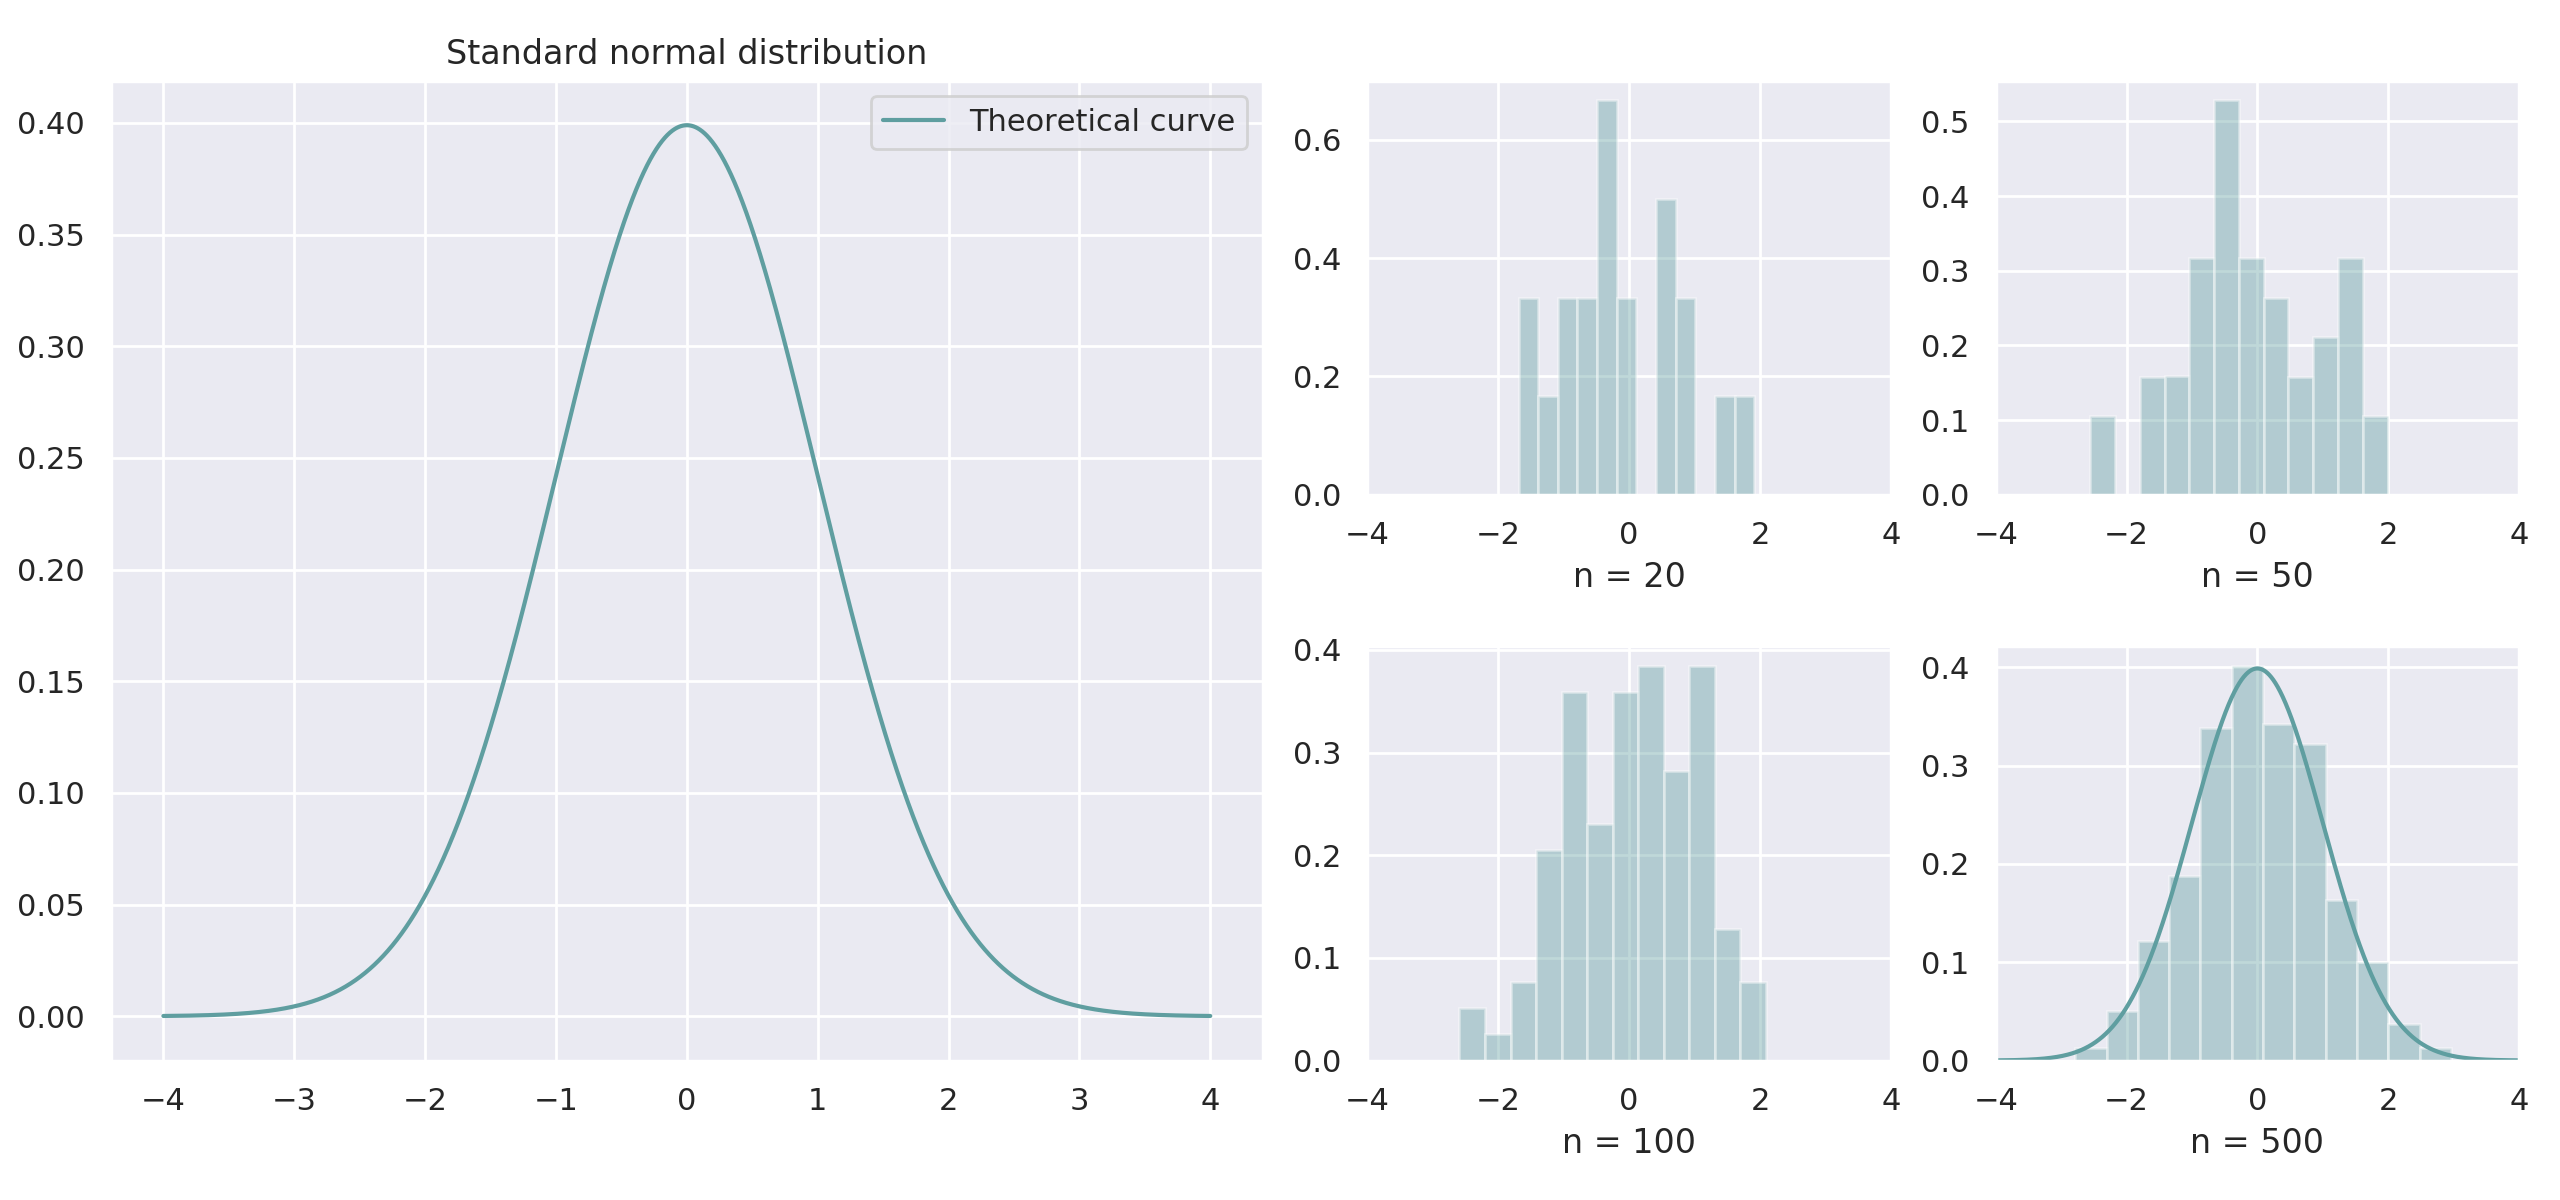
\includegraphics[width=16.cm, height=7.8cm]{norm_th}
\end{figure}

\textbf{Равномерное распределение} на отрезке $[-\sqrt{3}, \sqrt{3}]$

\begin{figure}[h!]
\centering
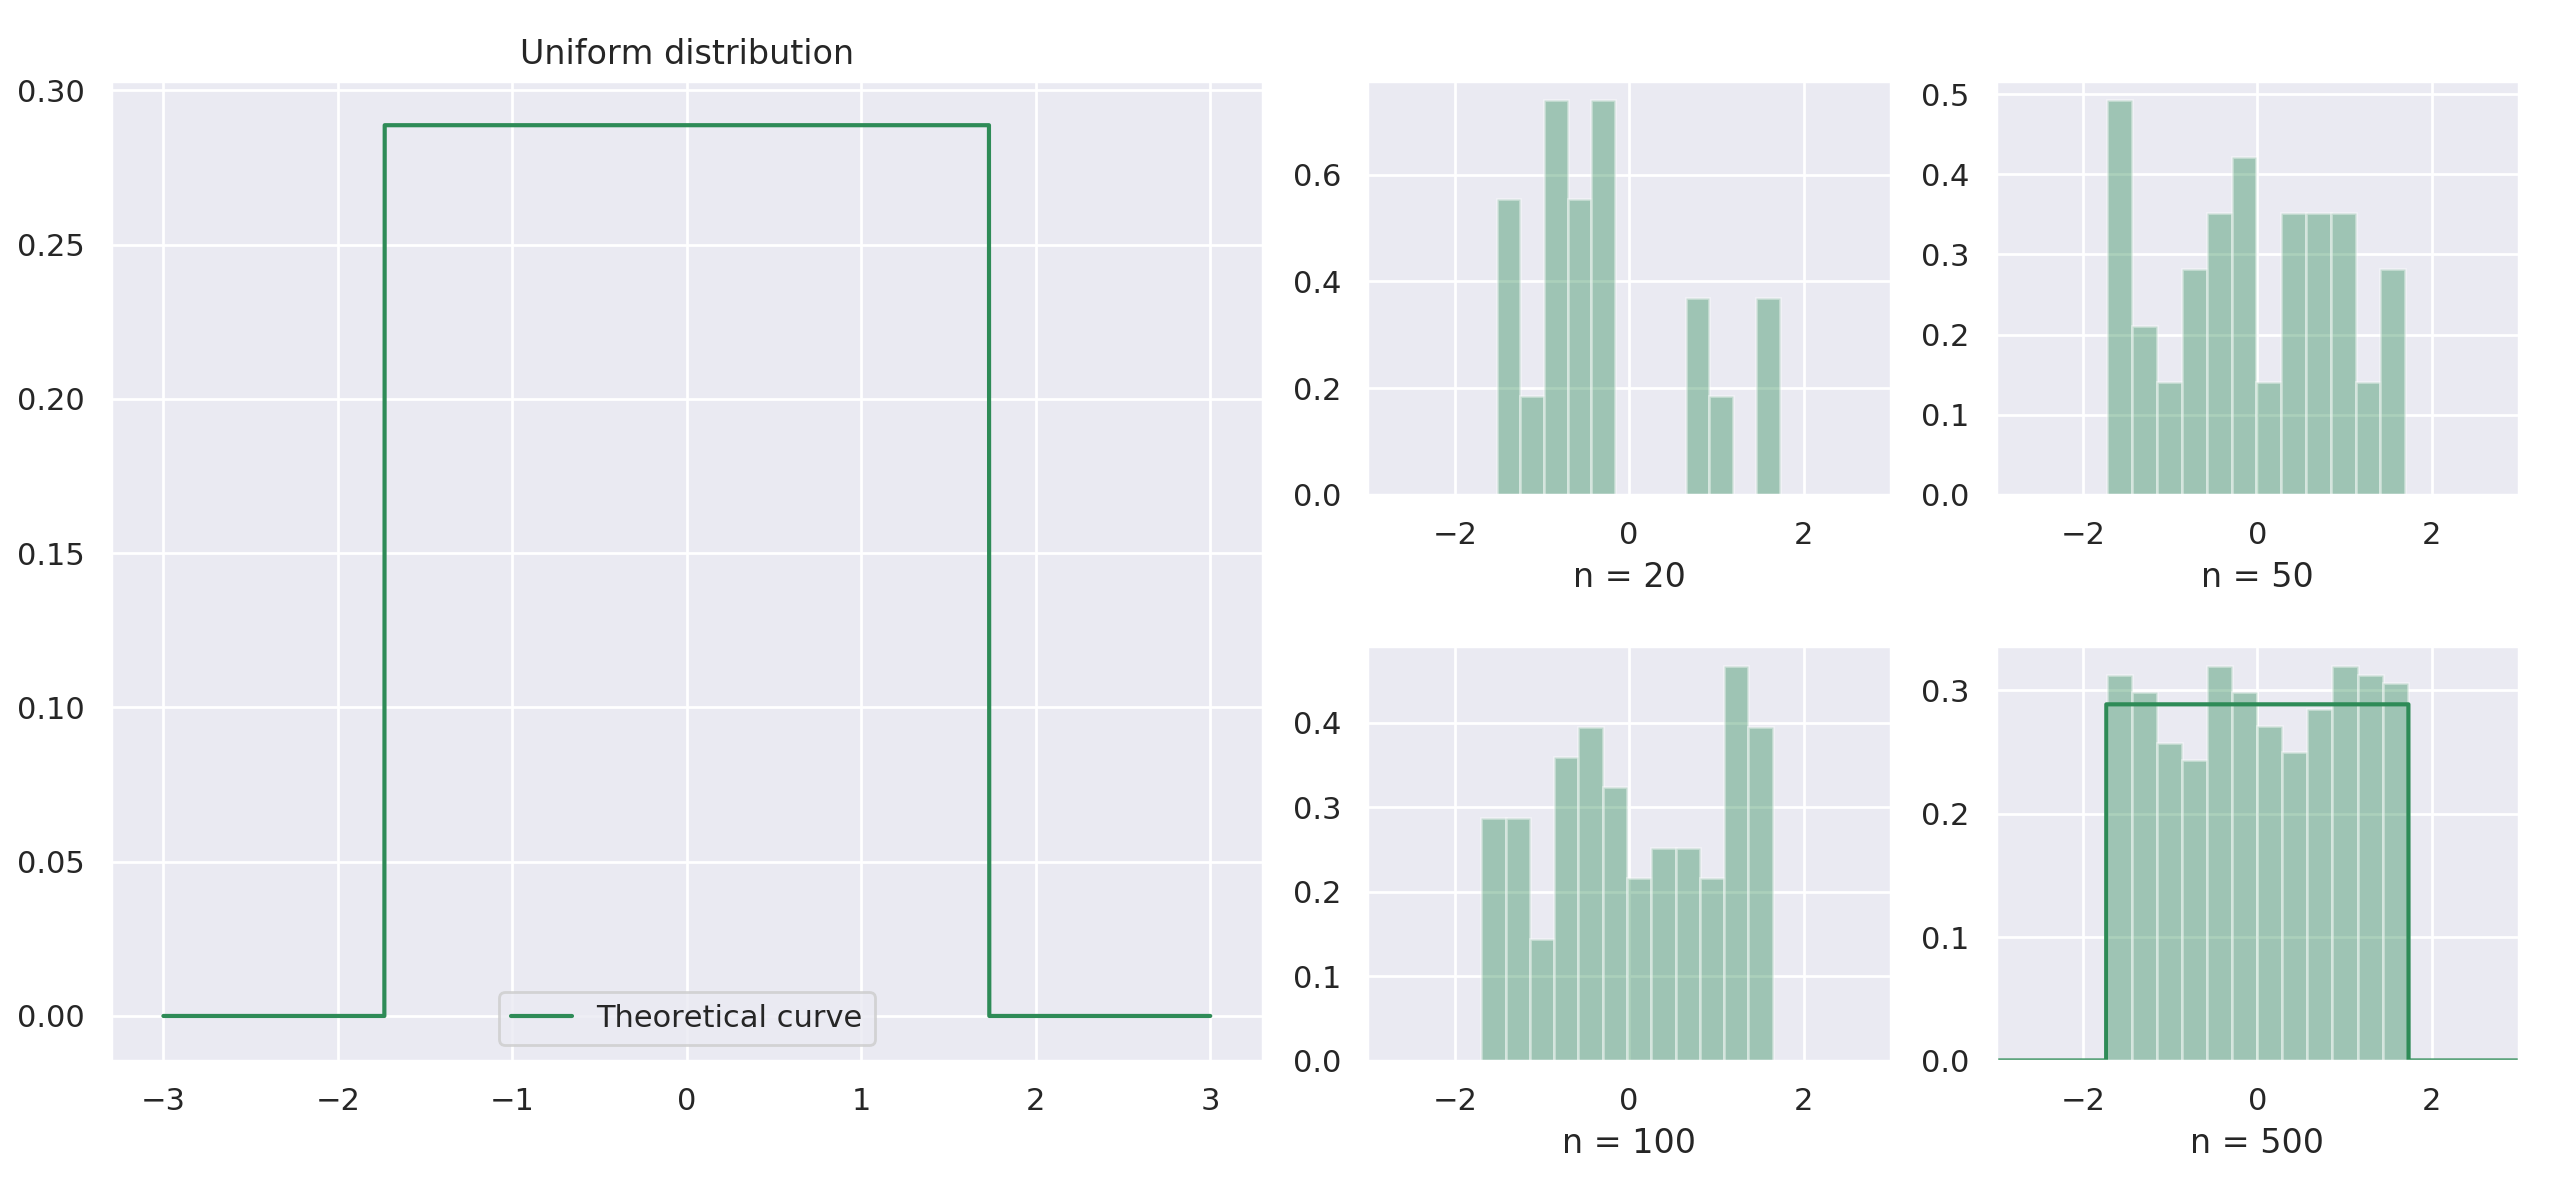
\includegraphics[width=16.cm, height=7.8cm]{uniform_th}
\end{figure}

\textbf{Распределение Коши} с параметрами 0, 1

\begin{figure}[h!]
\centering
\center{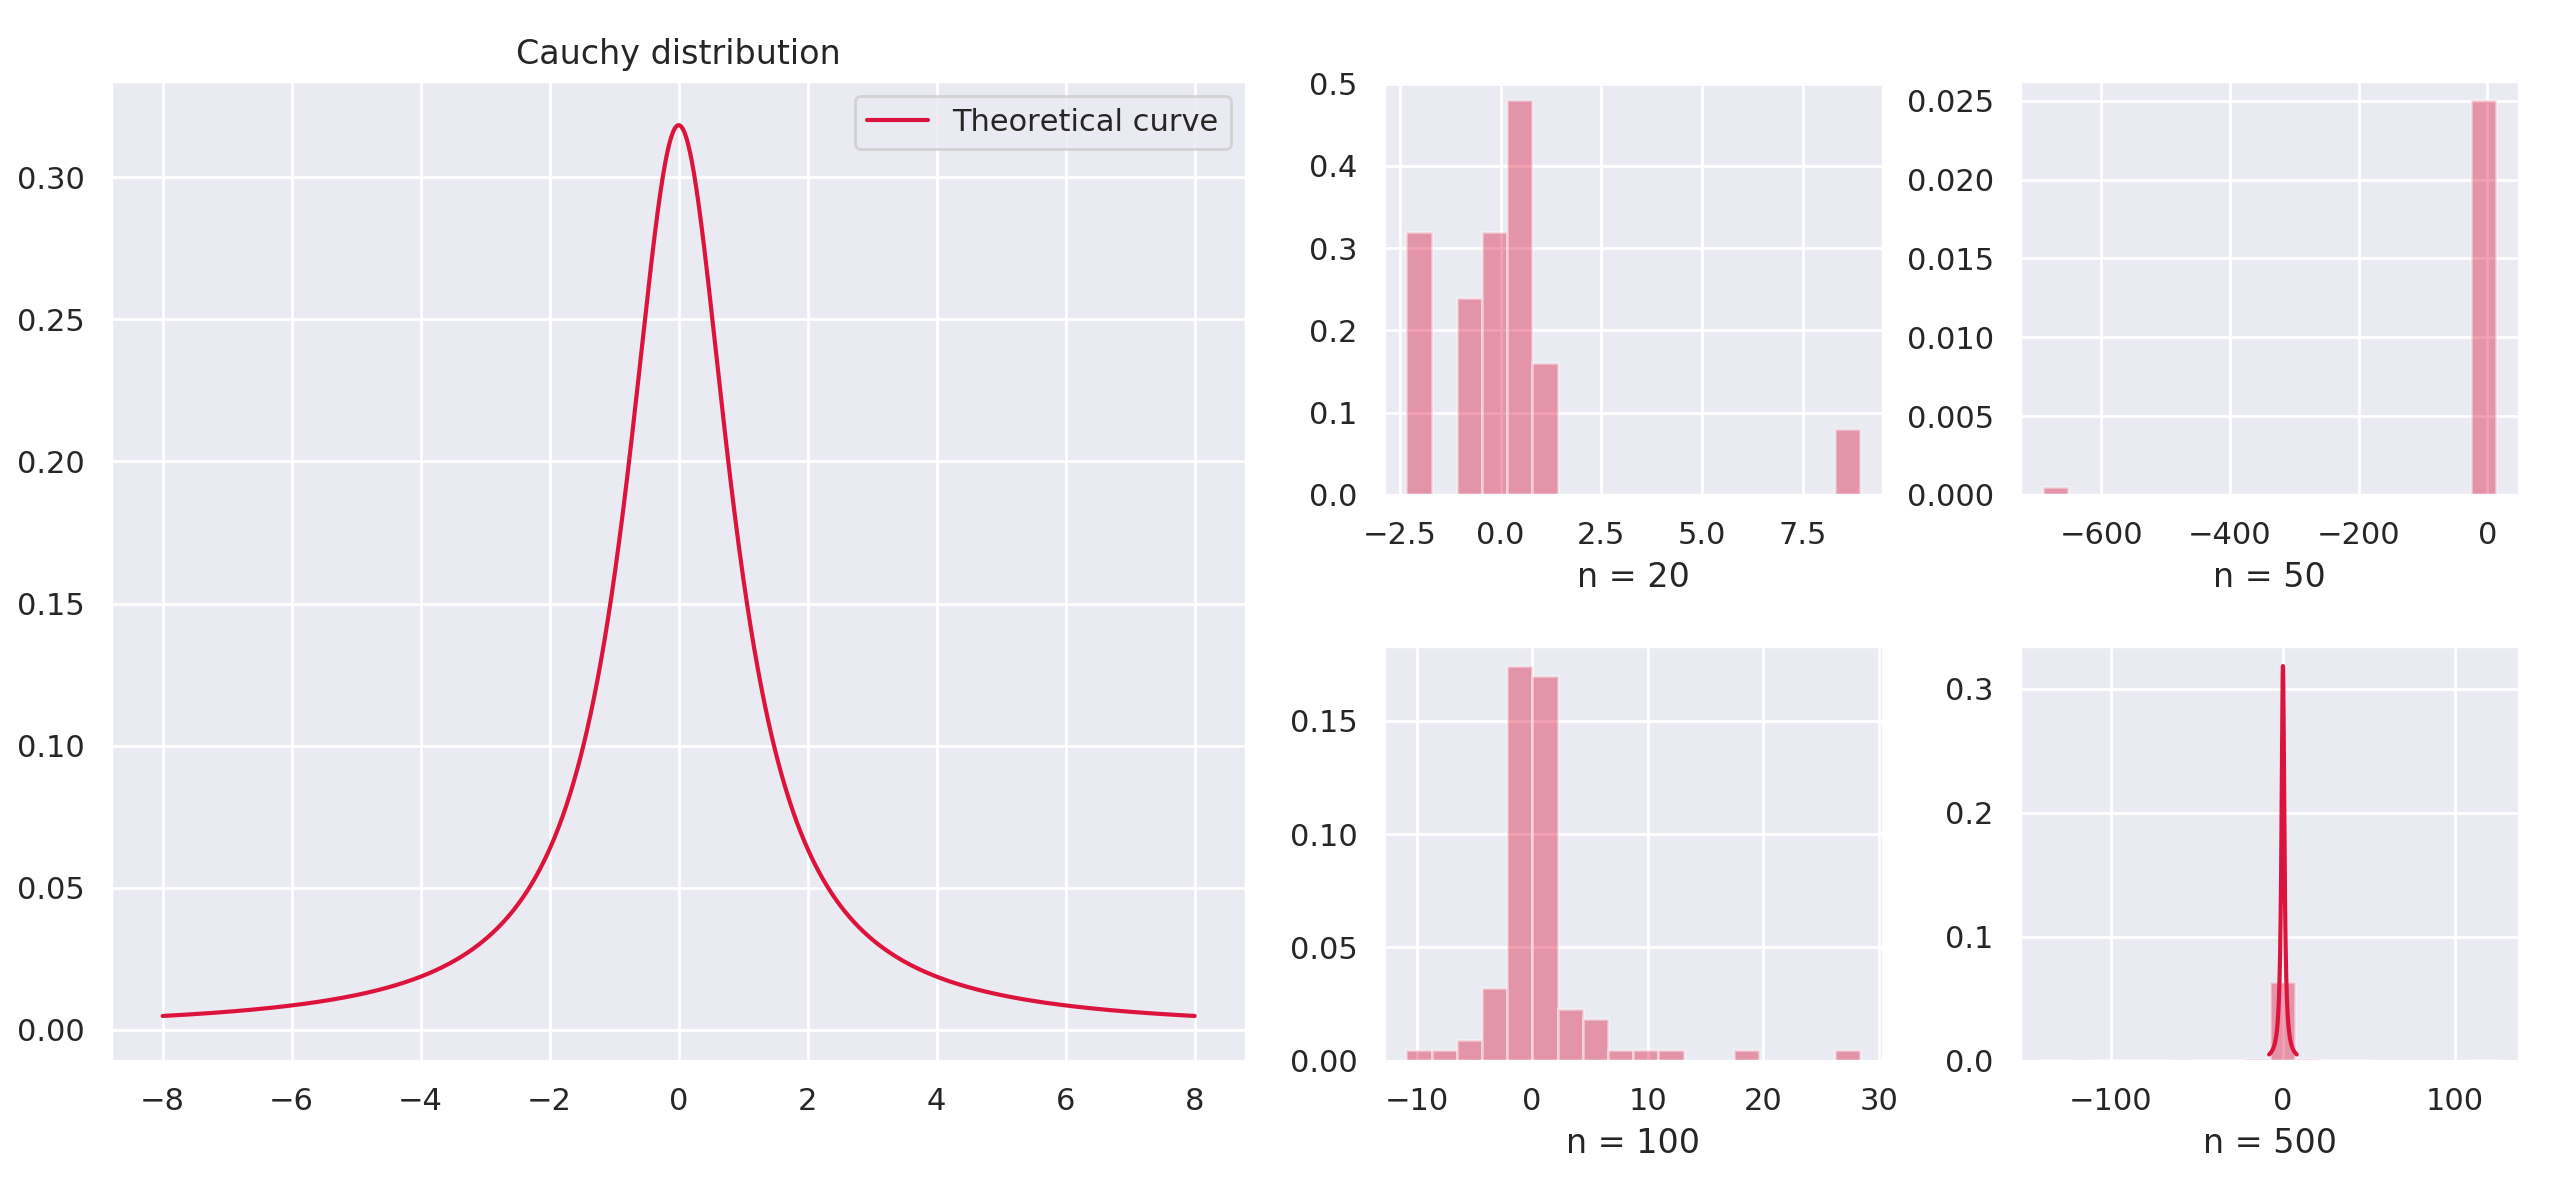
\includegraphics[width=16.8cm, height=8.5cm]{cauchy_th}}
\end{figure}

\textbf{Распределение Лапласа} с параметрами 0, $\frac{1}{\sqrt{2}}$

\begin{figure}[h!]
\centering
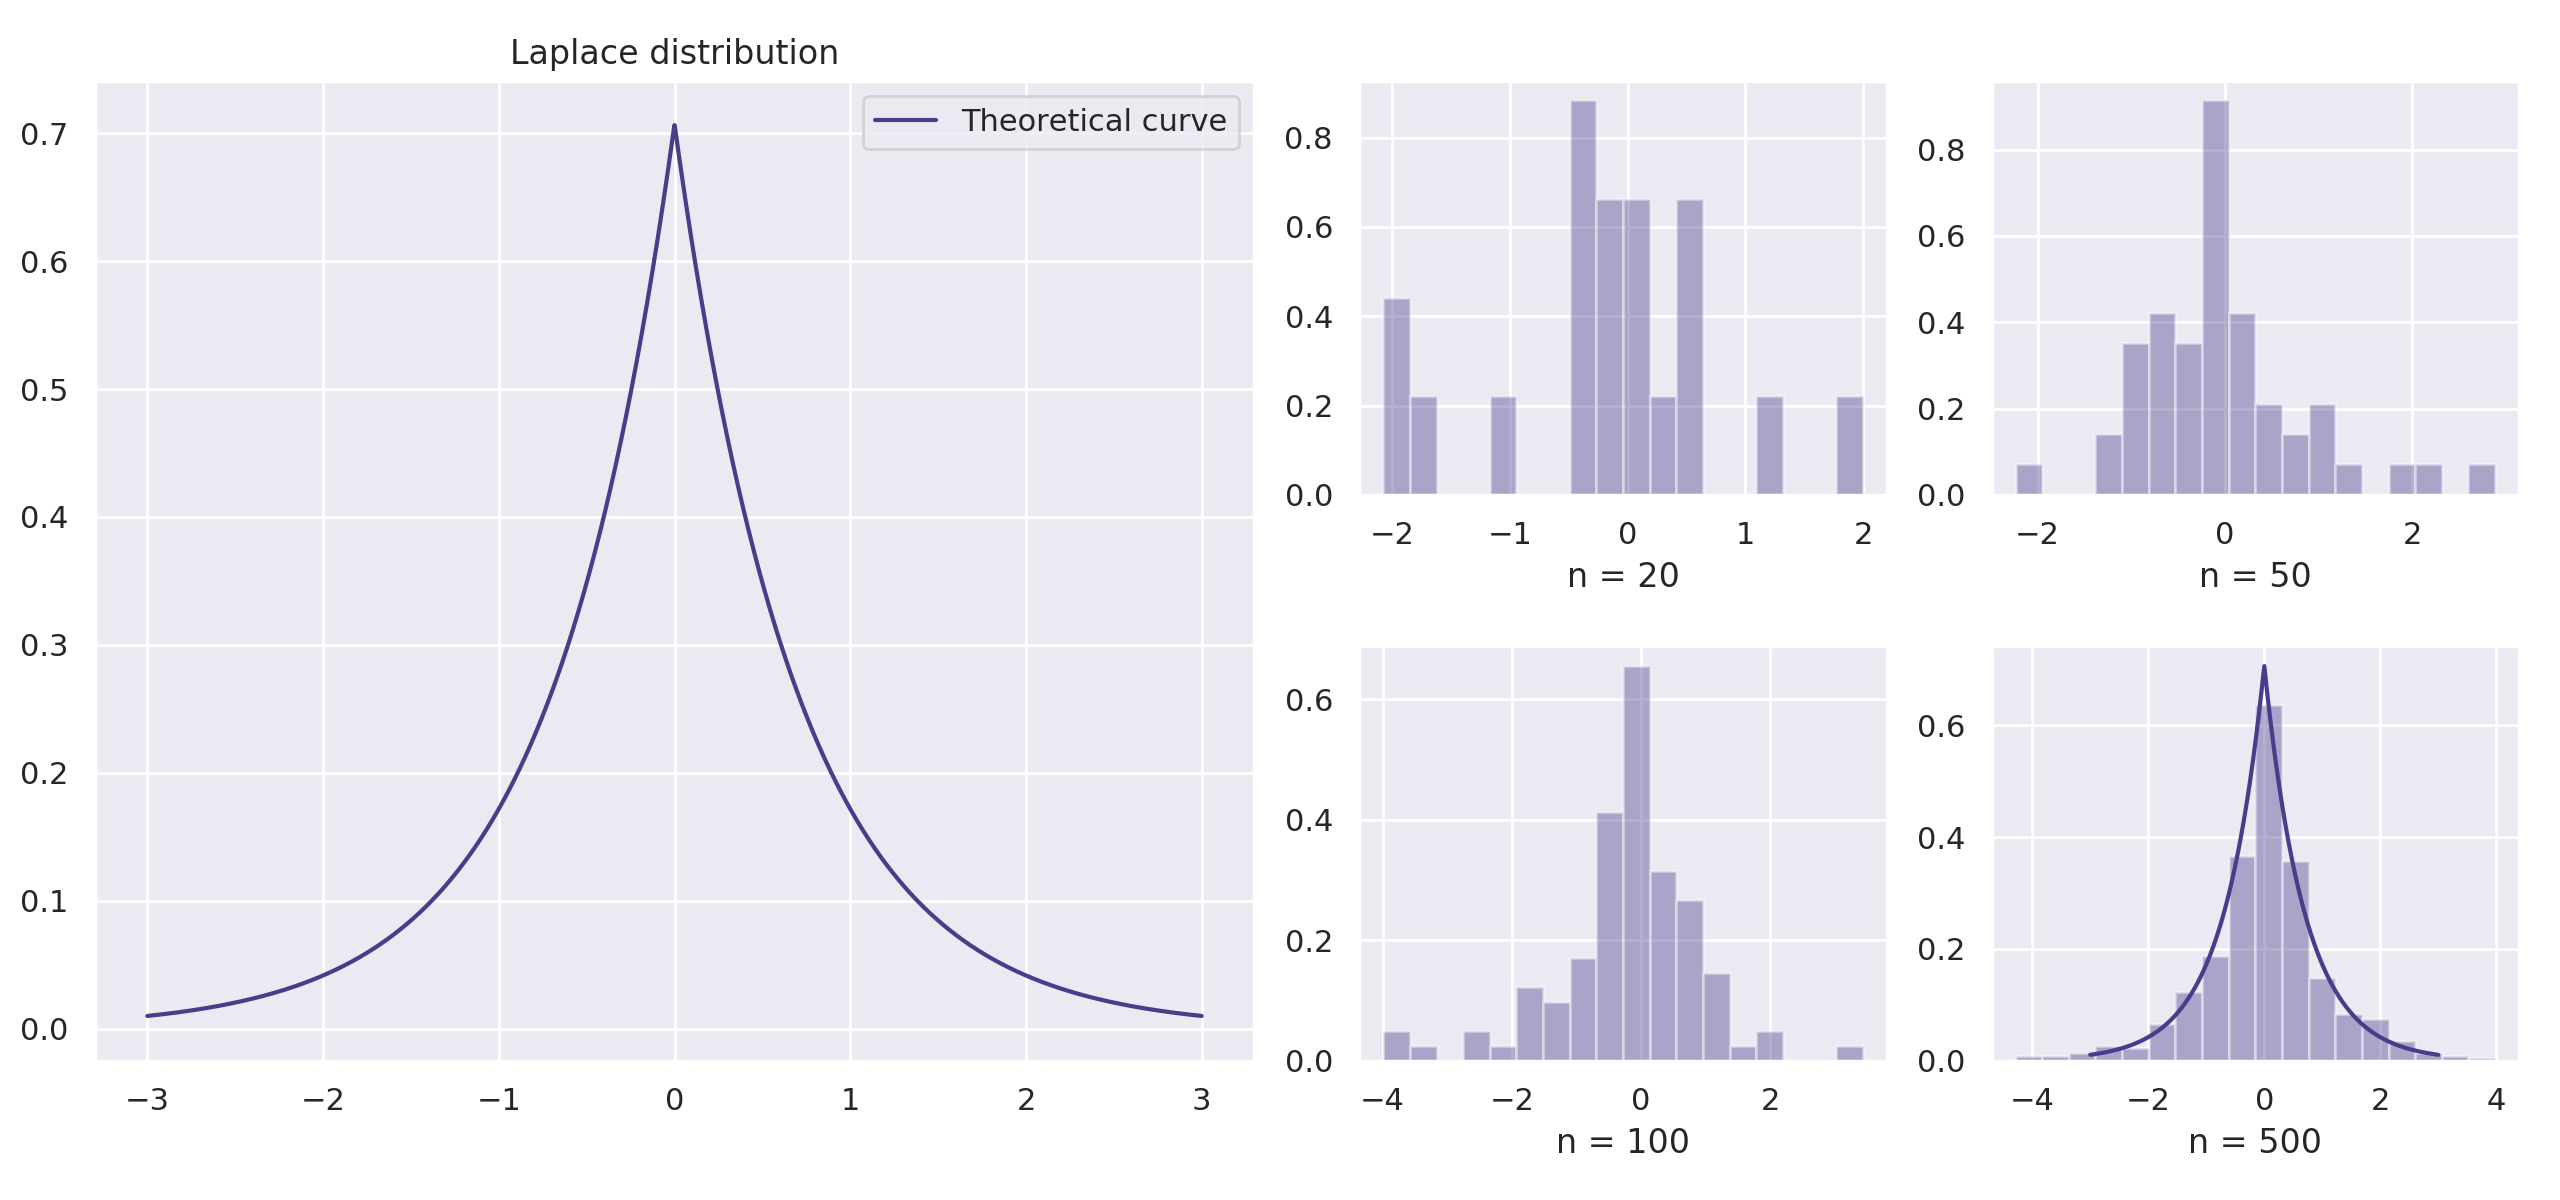
\includegraphics[width=16.8cm, height=8.5cm]{laplace_th}
\end{figure}

\indent{}
\textbf{Распределение Пуассона} с параметром $\lambda = 7$ \\
\indent{Выбор параметра обоснован стремлением распределения к нормальному при увеличении $\lambda$. Для наглядной визуализации  подходит число 7, к тому же являющееся числом Миллера, или предельной порцией информации, обрабатываемой человеком за раз (оригинальная статья - \cite{ms_2}). Этот факт является довольно символичным, учитывая область применения распределения Пуассона. }

\begin{figure}[h!]
\centering
\center{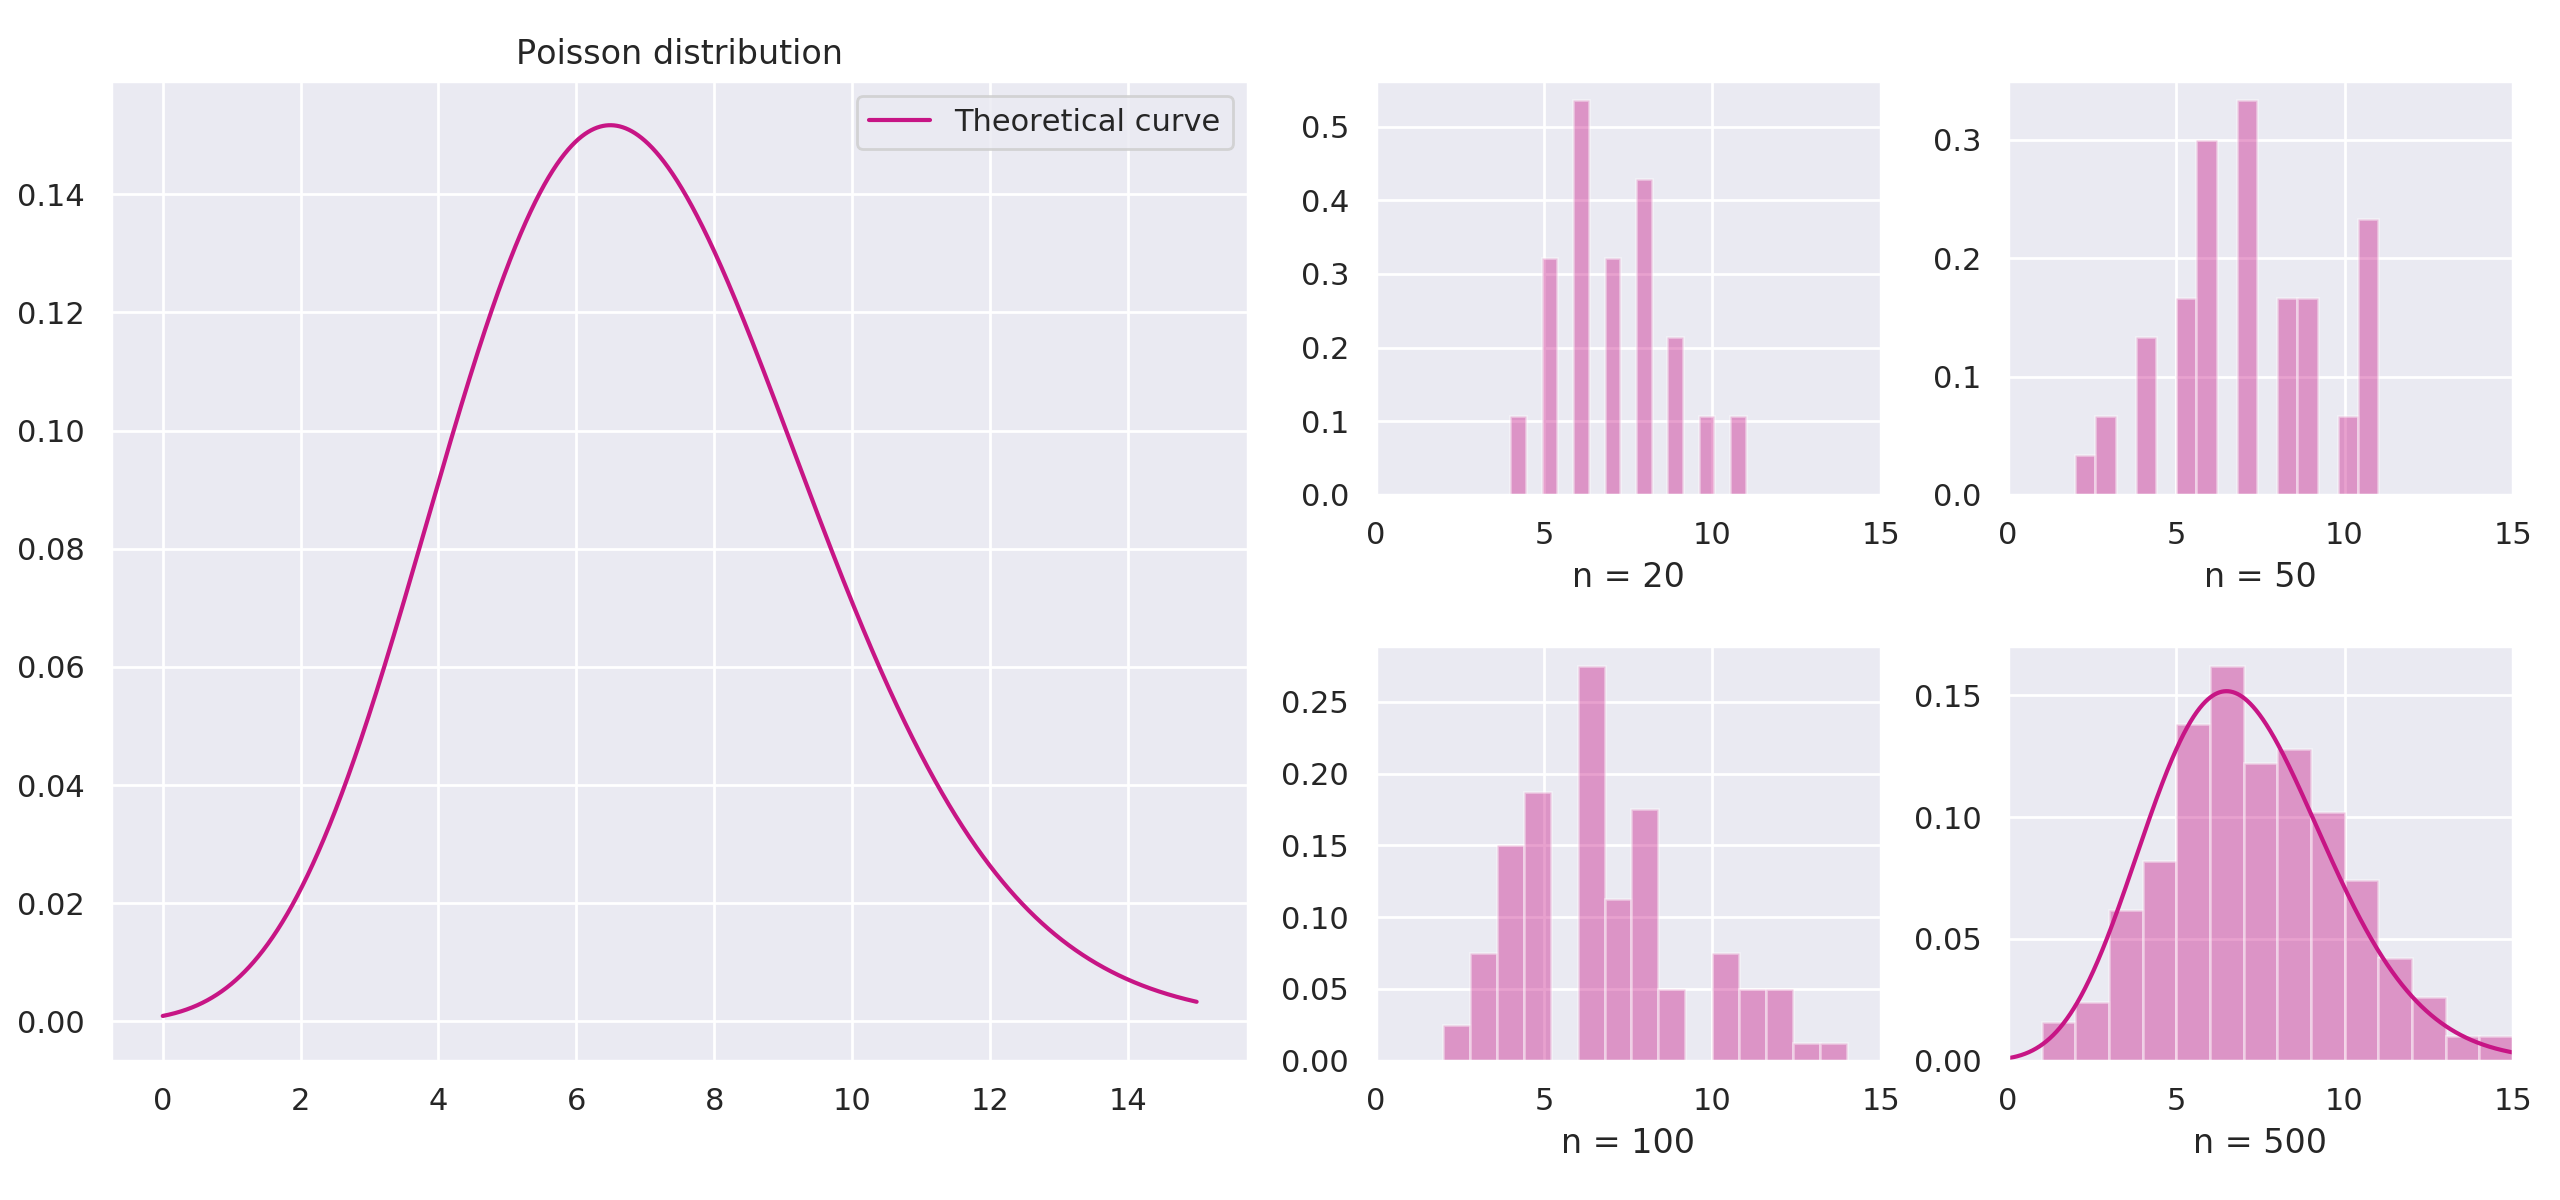
\includegraphics[width=16.cm, height=7.6cm]{poisson_th}}
\end{figure}

\indentПри достаточной мощности выборки из распределений (n = 100) гистограмму можно рассматривать как аналог плотности распределения непрерывной случайной величины.

%%%%%%%%%%%%%%%%%%%%%%%%%%%%%%%%%%%%%%%%%%

\newpage
\begin{thebibliography}{}
	\bibitem{ms_1} \textit{Кадырова Н. О.} Теория вероятностей и математическая статистика. Статистический анализ данных: учеб. пособие / \textit{Н. О. Кадырова, Л. В. Павлова, И. Е. Ануфриев.} - СПб.: Изд-во Политехн. ун-та, 2010. -54с.
	\bibitem{ms_2} \textit{Miller, G. A.} The magical number seven, plus or minus two: Some limits on our capacity for processing information. Psychological Review. 1956; 63:81–97.
\end{thebibliography}


\end{document}{}